\documentclass[14pt,a4paper]{scrartcl}
\usepackage[utf8]{inputenc}
\usepackage{ragged2e}
\usepackage[english,russian]{babel}
\usepackage{misccorr,color,ragged2e,amsfonts,amsthm,graphicx,systeme,amsmath,mdframed,lipsum}
\renewcommand\qedsymbol{$\blacksquare$}
\renewcommand*{\proofname}{\text{Доведення}}
\theoremstyle{definition}
\newtheorem{defo}{Означення}[section]
\newtheorem*{teo}{Теорема}
\newtheorem*{example}{Приклад}
\theoremstyle{remark}
\newtheorem*{remark}{Зауваження}
\theoremstyle{definition}
\newtheorem*{consequence}{Наслідок}
\theoremstyle{definition}
\newtheorem{statement}{Утверждение}[section]
\newmdtheoremenv{boxteo}{Теорема}[section]
\setlength\parindent{0pt}
\DeclareMathOperator*\lowlim{\underline{lim}}
\DeclareMathOperator*\uplim{\overline{lim}}


% Default fixed font does not support bold face
\DeclareFixedFont{\ttb}{T1}{txtt}{bx}{n}{12} % for bold
\DeclareFixedFont{\ttm}{T1}{txtt}{m}{n}{12}  % for normal

% Custom colors
\usepackage{color}
\definecolor{deepblue}{rgb}{0,0,0.5}
\definecolor{deepred}{rgb}{0.6,0,0}
\definecolor{deepgreen}{rgb}{0,0.5,0}

\usepackage{listings}

% Python style for highlighting
\newcommand\pythonstyle{\lstset{
language=Python,
basicstyle=\ttm,
otherkeywords={self},             % Add keywords here
keywordstyle=\ttb\color{deepblue},
emph={MyClass,__init__},          % Custom highlighting
emphstyle=\ttb\color{deepred},    % Custom highlighting style
stringstyle=\color{deepgreen},
frame=tb,                         % Any extra options here
showstringspaces=false            %
}}

\definecolor{javared}{rgb}{0.6,0,0} % for strings
\definecolor{javagreen}{rgb}{0.25,0.5,0.35} % comments
\definecolor{javapurple}{rgb}{0.5,0,0.35} % keywords
\definecolor{javadocblue}{rgb}{0.25,0.35,0.75} % javadoc

\lstset{language=C++,
basicstyle=\ttfamily,
keywordstyle=\color{javapurple}\bfseries,
stringstyle=\color{javared},
commentstyle=\color{javagreen},
morecomment=[s][\color{javadocblue}]{/**}{*/},
numbers=left,
numberstyle=\tiny\color{black},
stepnumber=2,
numbersep=10pt,
tabsize=4,
showspaces=false,
showstringspaces=false}


% Python environment
\lstnewenvironment{python}[1][]
{
\pythonstyle
\lstset{#1}
}
{}

% Python for external files
\newcommand\pythonexternal[2][]{{
\pythonstyle
\lstinputlisting[#1]{#2}}}

% Python for inline
\newcommand\pythoninline[1]{{\pythonstyle\lstinline!#1!}}
%
% \begin{python}
% class MyClass(Yourclass):
%     def __init__(self, my, yours):
%         bla = '5 1 2 3 4'
%         print bla
% \end{python}

\begin{document}



\def\be{\begin{equation}}
\def\ee{\end{equation}}
\def\bd{\begin{defo}}
\def\ed{\end{defo}}
\def\bbt{\begin{boxteo}}
\def\ebt{\end{boxteo}}
\begin{center}
Розрахункова робота № 2 \\
	Терещенко Денис КА-96 \\
	Варіант - 27
\end{center}

1,27, Знайти площу фігури, що обмежена даними лініями.

$$
y = \sin{(x)} \quad y = \cos{(x)} \quad x=0, (x\leq 0)
$$
\begin{center} 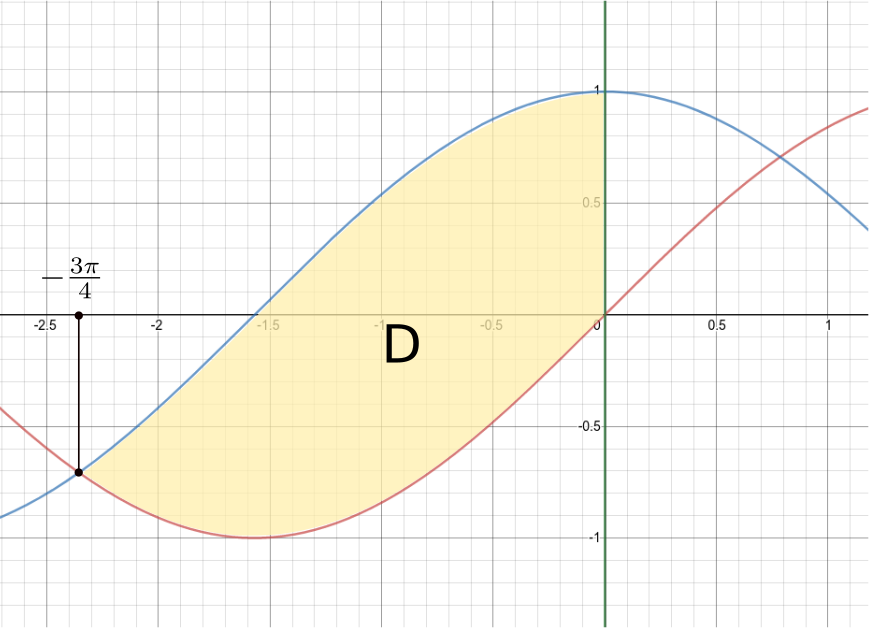
\includegraphics[scale=0.5]{1.png} \end{center}
Побудуємо задані криві. З графіка видно, що площа фігури $D$: $S_D =  \iint\limits_{D}{dxdy}$. З рівняння $\sin{(x)} = \cos{(x)}$ одна з точок перетину $x = \frac{-3\pi}{4} $. Тоді множину D можна представити як $D = \left\lbrace x \in [\frac{-3\pi}{4}; 0 ]; \sin{(x)} \leq y \leq \cos{(x)}   \right\rbrace $. Обчислимо:

$$
S_D =  \iint\limits_{D}{dxdy} =  \int\limits_{- \frac{3\pi}{4} }^{ 0}{dx  \int\limits_{\sin{(x)} }^{ \cos{(x)} }{dy}} = \int\limits_{- \frac{3\pi}{4} }^{ 0}{ \cos{(x)}- \sin{(x)} dx } = \sqrt{2} + 1
$$

\pagebreak

2.27. Пластина $D$ обмежена кривими; $\mu$ - щільність. Знайти масу пластини.
$$
\Bigg[
\begin{gathered}
 D: x = 2, y=0, y^2 = x/2, (y\geq 0)\\
 \mu = 4x + 6y^2
\end{gathered}
$$
\begin{center} 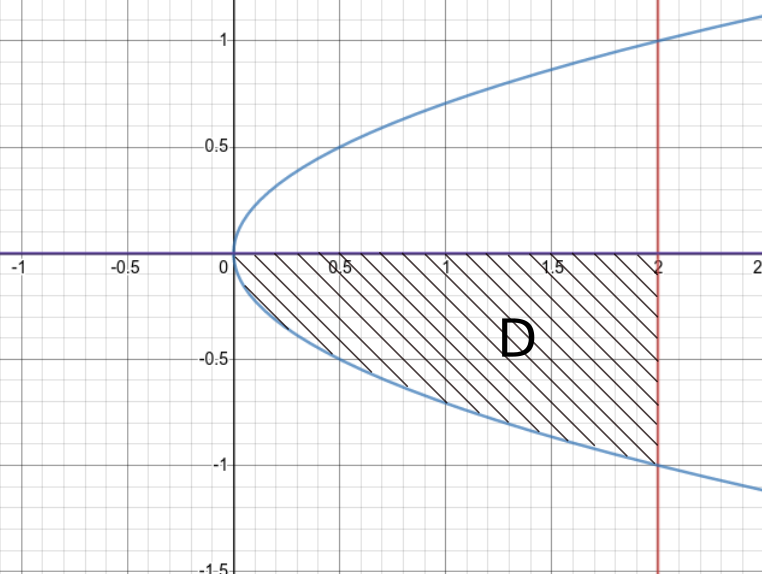
\includegraphics[scale=0.5]{2.png} \end{center}
Область $D$ зобразимо на графіку.
Вона дорівнює:
$D_{x,y}= \left\lbrace x \in[0,2] ; -\sqrt{x/2} \leq y\leq 0 \right\rbrace $.
Формула для обчисленням маси пластини: $ M(D) =  \iint\limits_{D}^{}{\mu(x,y )dx dy}$.
$$
M(D) =  \iint\limits_{D}^{}{\mu(x,y )dx dy} =  \int\limits_{0}^{2}{dx \int\limits_{- \sqrt{	\frac{x}{2} 	}}^{ 0}{(4x+6y^2) dy}}=  \int\limits_{0}^{2}{
\dfrac{5x^\frac{3}{2}}{\sqrt{2}}dx
} =\sqrt{2}x^\frac{5}{2} \Bigg|_{0}^2= 8
$$

\pagebreak

3.27. Знайти об'єм тіла, яке задано поверхнями, що обмежують його.
$$
\begin{gathered}
z = 28(x^2+ y^2)+ 3\\
z = 56y + 3
\end{gathered}
$$
\begin{center} 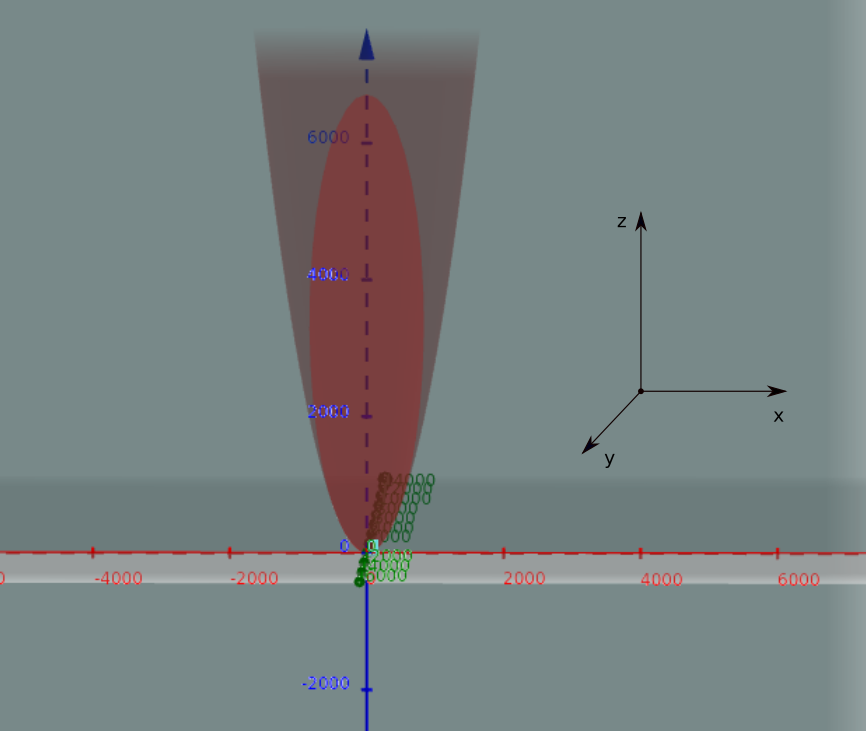
\includegraphics[scale=0.5]{4.png} \end{center}
Зобразимо отриману фігуру на графіку. Бачимо, що необхідно визначити об'єм між похилою площиною та параболоїдом. У перетині площини та параболоїда лежить еліпс. Буде зручно розглянути проекцію фігур на $YOZ$.
$$
\begin{gathered}
 \text{В такому разі маємо:}\\
 \text{З умови } x =0:\\
 A = (0, 0, 3)\\
 B = (0, 2, 115)\\
 D - \text{область}
\end{gathered}
\qquad \qquad
\begin{gathered}
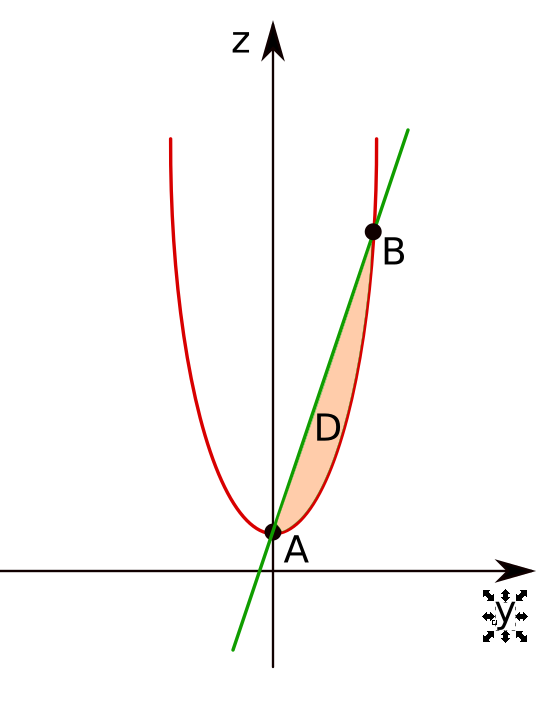
\includegraphics[scale=0.27]{3.png}
\end{gathered}
$$
Для знаходження об`єму будемо інтегрувати за площиною $D$ вираз $x_{\text{вих}} - x_{\text{вх}}$, де з умови та графіка знаходимо:
$$x_{\text{вих}}= \sqrt{ \frac{z-3}{28} - y^2} \qquad x_{\text{вх}} = - \sqrt{ \frac{z-3}{28} - y^2}$$
Тоді остаточно, приходимо до обчислення об'єму \\ $D = \left\lbrace y \in [0, 2]; 28y^2 +3 \leq  z \leq  56y + 3 \right\rbrace $:
$$
V(\Sigma) =  2\iint\limits_{D}^{}{\sqrt{ \frac{z-3}{28} - y^2}dydz} =  2\int\limits_{0}^{2}{dy  \int\limits_{28y^2 +3}^{ 56y + 3}{\sqrt{ \frac{z-3}{28} - y^2}dz}} =
$$
$$
= \int\limits_{0}^{2}{ \left( \dfrac{112\left(\frac{z-3}{28}-y^2\right)^\frac{3}{2}}{3} \right) \Bigg|_{28y^2 +3}^{56y + 3} dy} =
\int\limits_{0}^{2}{ -\dfrac{112\left(y-2\right)y\sqrt{2y-y^2}}{3} dy} =
$$
Подальше інтегрування та обчислення було досить об'ємним, але чисельне значення збіглося з обчисленням, виконаним алгоритмом на Python. На початку потрібно було перейти до циліндричних координат, це спростило би умову.
$$
= -\dfrac{56\left(-\frac{y\left(2y-y^2\right)^\frac{3}{2}}{4}+\frac{\left(2y-y^2\right)^\frac{3}{2}}{4}-\frac{3y\sqrt{2y-y^2}}{8}+\frac{3\sqrt{2y-
y^2}}{8}+\frac{3\arcsin\left(\frac{2-2y}{2}\right)}{8}\right)}{3}
\Bigg|_0^2
= 7 \pi
$$


\pagebreak


4.27. Знайти об'єм тіла, яке задано поверхнями, що обмежують його.
$$
x+y = 8 \qquad y = \sqrt{4x} \qquad z=3y \qquad z =0
$$
Подубуємо задані площини. Фігура ``S'' - це фігура, об'єм якої треба знайти.
$$
\begin{gathered}
 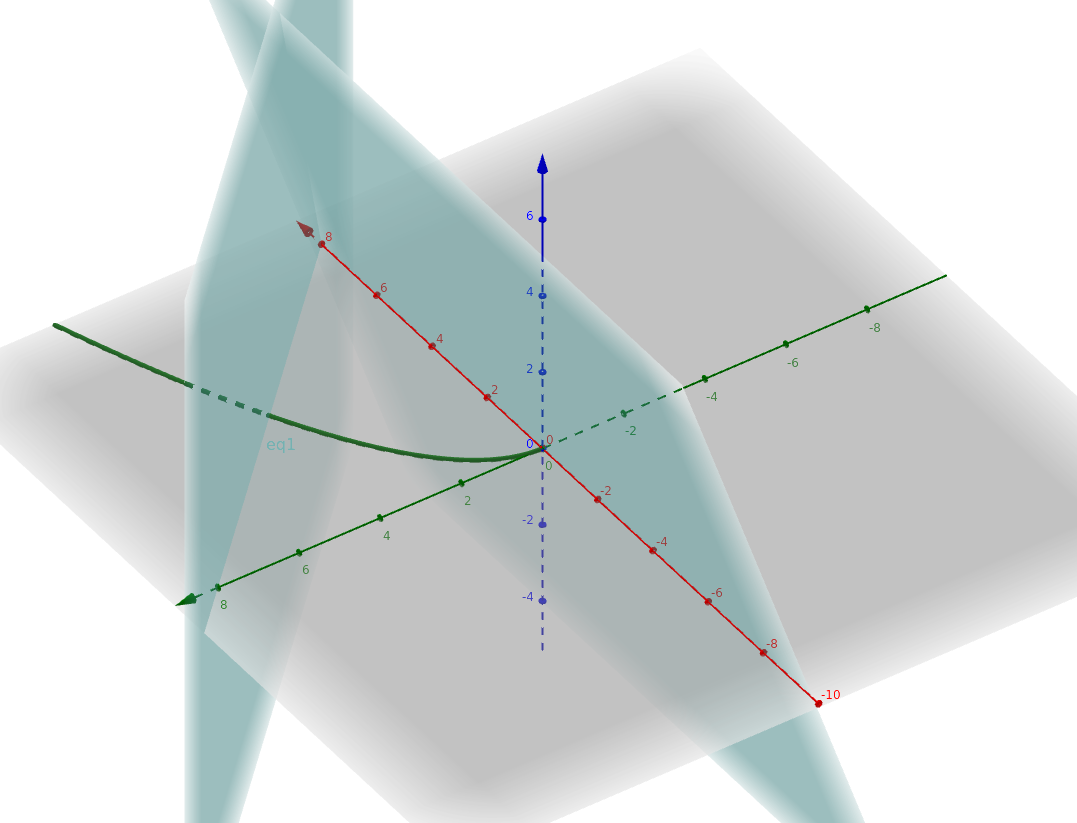
\includegraphics[scale=0.2]{5.png}
\end{gathered}\qquad
\begin{gathered}
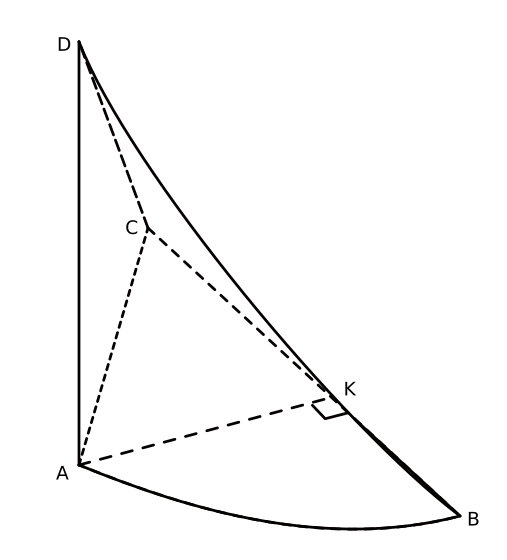
\includegraphics[scale=0.3]{6.png}
\end{gathered}
$$
Спочатку, спроектуємо фігуру на площину $XOY$. Отримаємо $ABC$. Тобто, об'єм дорвінює: $$V(S) =  \iiint\limits_{S}{dxdydz}  =  \int\limits_{0}^{ 8}{ dx \int\limits_{2\sqrt{x}}^{ 8-x}{dy  \int\limits_{0}^{ 3y}{dz}}}=  \int\limits_{0}^{ 8}{ dx \int\limits_{2\sqrt{x}}^{ 8-x}{3ydy }}=$$
$$
=   \int\limits_{0}^{ 8}{ \dfrac{3x^2-60x+192}{2} dx } = \dfrac{x\left(x^2-30x+192\right)}{2} \Bigg|_{0}^{8} = 64
$$

\pagebreak

5.27. Тіло $\Omega$ обмежено поверхнями, $\mu$ - щільність. Знайти масу тіла.
$$
\begin{gathered}
x^2 + y^2 + z^2 = 9 \qquad x^2 + y^2 = 4\qquad x^2 + y^2 \leq 4\\
z = 0 \qquad z\geq 0 \qquad \mu = 2z
\end{gathered}
$$
\begin{center} 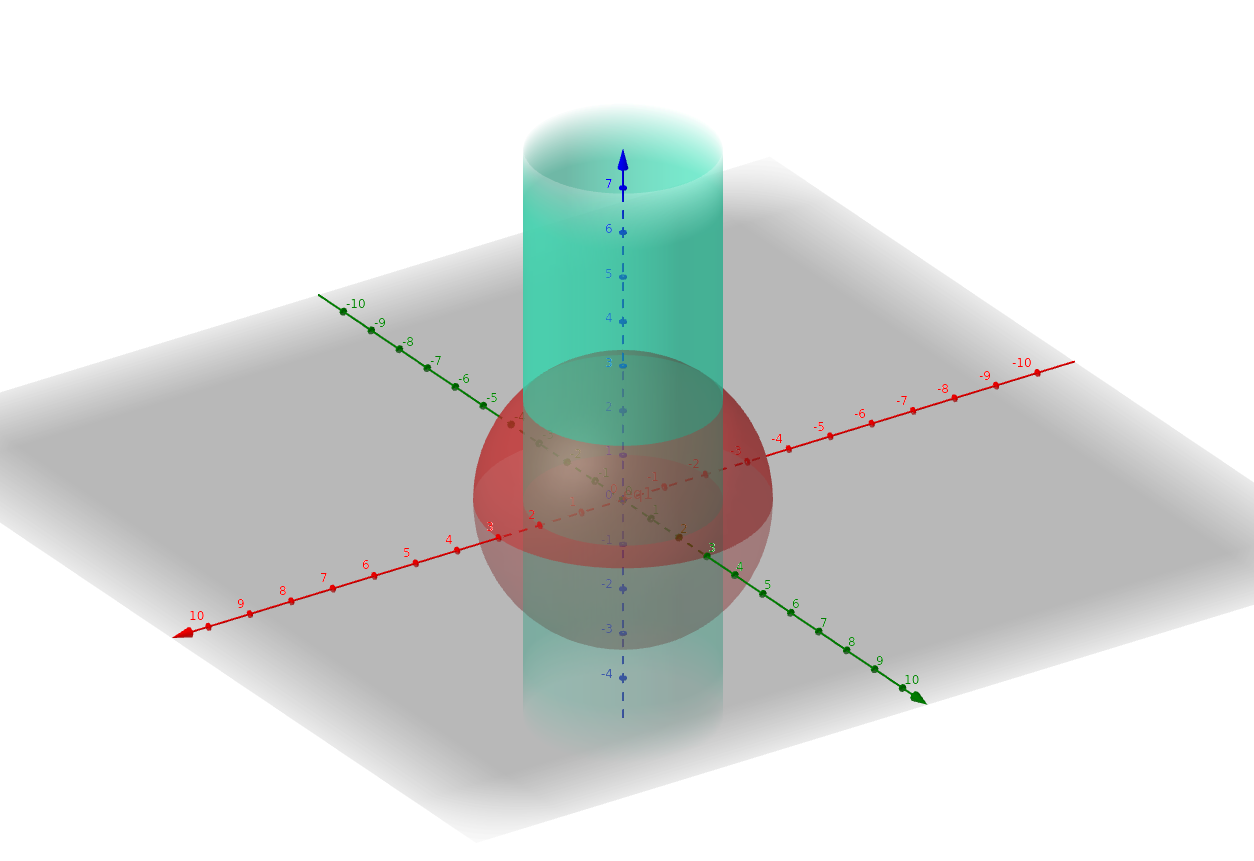
\includegraphics[scale=0.3]{7.png} \end{center}
Зобразимо задані площини. Неохідно знайти масу частини шара, вирізану циліндром. Для цього перейдемо в циліндричні координати.
$$
\left\lbrace
\begin{gathered}
  x = \rho \cos{(\varphi)}\\
	y = \rho \sin{(\varphi)}\\
	J = \rho\\
	x^2 + y^2 = \rho^2
\end{gathered}
 \right.\quad
 \Longrightarrow
 \quad
 \left\lbrace
 \begin{gathered}
   \rho^2 + z^2 = 9, z = \sqrt{9 - \rho^2}\\
 	\rho^2 = 4\quad (\rho^2 \leq 4)\\
 	z= 0 \quad(z\geq 0)
 \end{gathered}
  \right.\quad
$$

Масса шуканого тіла $\Omega$: $ M(\Omega) =  \iiint\limits_{\Omega}^{}{2zdxdydz}$
$$
 M(\Omega) = \int\limits_{0}^{2\pi}{ d \varphi \int\limits_{0}^{2}{  d\rho \int\limits_{0}^{ \sqrt{9 - \rho^2}}{2\rho z dz}}} =
 \int\limits_{0}^{2\pi}{ d \varphi \int\limits_{0}^{2}{ \rho(9-\rho^2) d\rho }} = 32 \pi
$$
\end{document}
